% !TeX spellcheck = en_US
\section{Graph visualization}\label{section:graph}

In this section, graph visualization window is described. Graph data is stored in .graph file. 
You can open this file by double clicking on it in workspace tree.

Preference graph is created from induced rules. Vertices of graph represents objects from test data file. 
Arcs represent outranking $S$ or non-outranking $S^{c}$ relations between objects. 
If an arc is present between vertices x and y, it means that pair (x,y) is covered by a decision rule which suggests assignment to relation $S$ or $S^{c}$ respective. 
Arcs can also be weighted, where weight is equal to satisfaction degree of preference relation.
Rule credibility is used for arc weight. 
If a pair of objects is covered by multiple rules, they credibilities are aggregated once arc weight equals maximum credibility.

\begin{figure*}[!ht] 
	\centering
	\makebox[\textwidth]{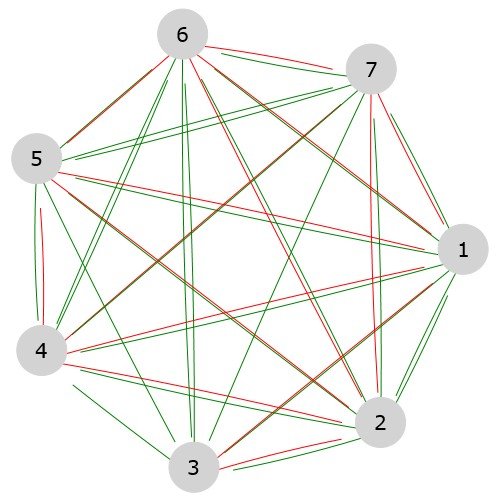
\includegraphics[width=.5\paperwidth]{raw/graph}}
	\caption{Graph visualization for Houses7}
\end{figure*}

For each pair of vertices (x,y), up to four relations can be satisfied:
\begin{itemize}
	\item $x S y$
	\item $x S^{c} y$
	\item $y S x$
	\item $y S^{c} y$
\end{itemize}

Relation type is marked with line color. Green is for outranking relation $S$ and red for non-outranking relation $S^{c}$. So relation $x S y$ will be represented as a green line between these two vertices.

All arcs are directed. Direction of an arc is marked using line ending. Lines end before target vertex. So $x S y$ relation will be drawn as a line from vertex $x$ to vertex $y$ with line ending slightly before $y$.

To improve arc visibility, only up to two arcs are drawn between vertices. In case of two relations: $x S y$, $x S^{c} y$ - just one arc with gray color will be drawn between $x$ and $y$. 
Same reduction is made for $y S x$, $y S^{c} x$.

You can navigate on graph by using scrollbars, as well as zoom in and zoom out by mouse wheel. You can also drag vertices to changing their position. If you click on a vertex, it will be selected and summary for arcs will be displayed in a tab below. All arc weights are displayed there in square brackets.

\begin{figure*}[!ht] 
	\centering
	\makebox[\textwidth]{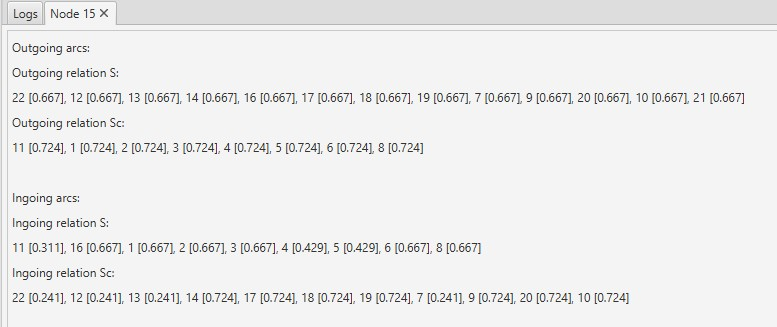
\includegraphics[width=.7\paperwidth]{raw/graph-arcs}}
	\caption{Vertex arcs for NotebooksVCcF with weights}
\end{figure*}


\vfill\newpage